\chapter{Experimento}\label{chapter:experimento}

Neste capítulo é apresentado o experimento realizado para a avaliação da proposta apresentada no Capítulo \ref{chapter:proposta}.
Para avaliar a proposta deste trabalho foi utilizada uma avaliação pela perspectiva do usuário, que segundo a definição de
\citeonline{shani2011evaluating} se encaixa em um Estudo com usuários. O algoritmo proposto foi incorporado ao ambiente
\adaptwebspace e avaliado em uma situação real de uso em um Minicurso de Algoritmos desenvolvido por \citeonline{santos2017addie}.
Na Seção \ref{section:planejamento-experimento} é descrito o ambiente \adaptwebspace no qual a proposta foi incorporada,
as mudanças realizadas no ambiente para o experimento, o objetivo do experimento e o teste piloto realizado. A Seção
\ref{section:execucao-experimento} descreve o experimento que foi realizado e a Seção \ref{section:analise-experimento} apresenta
as análises realizadas no uso do Sistema de Recomendação (SR) e no questionário aplicado.

\section{Planejamento}\label{section:planejamento-experimento}

Essa seção explica em mais detalhes o ambiente \adaptweb, o Minicurso de Algoritmos e Linguagem de Programação utilizado
para o experimento, as mudanças propostas para o ambiente para a realização do experimento e os detalhes do experimento
realizado, tais como as hipóteses do experimento e os critérios para divisão dos alunos nos dois grupos.

\subsection{Descrição do Ambiente \adaptweb}

O \adaptwebspace (Ambiente de Ensino-Aprendizagem Adaptativo na Web) é um sistema \textit{open source}
que consiste em um AVA capaz de adaptar o conteúdo, a apresentação e a navegação em determinado curso às características
e preferências do aluno \cite{gasparini2009adaptweb}. A Seção \ref{subsection:estrutura-adaptweb} apresenta a Estrutura Geral do
\adaptweb.

\subsubsection{Estrutura do \adaptweb}\label{subsection:estrutura-adaptweb}

A estrutura do \adaptwebspace é composta por quatro módulos: (1) o módulo de autoria; (2) o
módulo de armazenamento em XML (Extensible Markup Language); (3) o módulo de adaptação do conteúdo baseado no modelo do
usuário e (4) o módulo de interface adaptativa \cite{gasparini2003interface}, conforme pode ser visto na Figura
\ref{fig:adaptweb-arquitetura}.

\begin{figure}[htb]
  \caption{\label{fig:adaptweb-arquitetura}Estrutura do \adaptweb}
  \begin{center}
      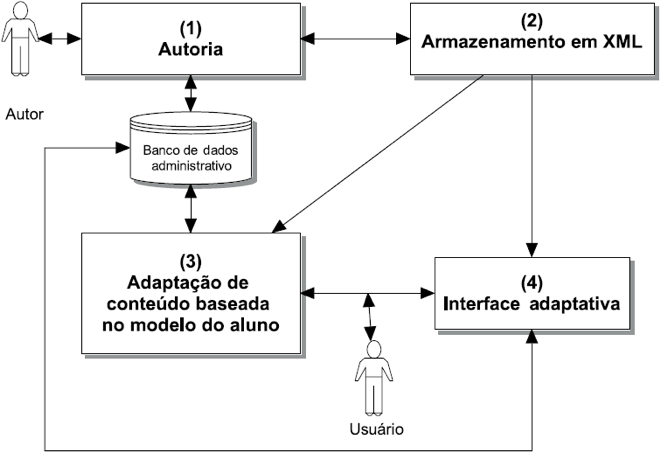
\includegraphics[scale=1.0]{./Figuras/adaptweb-arquitetura.png}
  \end{center}
  \legend{Fonte: \citeonline{gasparini2003interface}}
\end{figure}

O módulo de autoria (1) consiste na organização do conteúdo instrucional a ser disponibilizado para o aluno, sendo que
este conteúdo pode ter arquivos classificados como conceito, exemplos, exercícios e materiais complementares
\cite{gasparini2003interface}. Ao criar um conteúdo no sistema, o autor pode definir para quais cursos e disciplinas
deseja que o conteúdo ou arquivo esteja disponível. Isto significa que um aluno de um Curso X e de outro Curso Y,
matriculados em uma mesma disciplina, podem ter conteúdos distintos, conforme definido pelo professor. Por exemplo, a
disciplina de Cálculo I pode ser oferecida para os cursos de Ciência da Computação e Engenharia Elétrica e sua
abrangência e profundidade pode ser distinta para cada curso.

Em \citeonline{de2015sistema}, foi proposta uma nova categoria para os conteúdos chamada Links de Apoio. Esses Links de Apoio
são links externos ao ambiente \adaptwebspace que são cadastrados pelo professor como um
material alternativo de estudo e não estão diretamente atrelados a nenhum conceito em específico. O objetivo foi criar
uma nova categoria de materiais que poderia ser recomendada para o usuário a qualquer momento de sua interação.

O módulo de armazenamento em XML (2) é responsável por organizar os conteúdos e arquivos disponibilizados pelo autor em
um arquivo XML \cite{gasparini2003interface}. É utilizada a representação através de XML devido à sua alta
flexibilidade, oferecendo a estruturação dos documentos de forma independente da apresentação.

O módulo de adaptação do conteúdo baseado no modelo do aluno (3) é responsável por adaptar o conteúdo da disciplina
para cada curso. Por fim, o módulo de interface adaptativa (4) é responsável pela adaptação da navegação e da
apresentação da interface do ambiente de acordo com o curso, preferências do modo de navegação (modo tutorial ou livre)
e o conhecimento do usuário \cite{gasparini2003interface}.

\subsubsection{Sistema de Recomendação no \adaptweb}

Na Seção \ref{subsection:estrutura-adaptweb} foi apresentada a estrutura do ambiente \adaptweb, que possui quatro categorias
de materiais para cada conteúdo. Além disso, existe uma outra categoria chamada Links de Apoio com o propósito de ser um
material auxiliar e que pode ser recomendado a qualquer momento para o usuário.

Fazendo uma relação da estrutura do \adaptwebspace com o algoritmo proposto no Capítulo \ref{chapter:proposta}, os itens
das categorias Conceito, Materiais Complementares e os próprios Links de Apoio são considerados para a composição do
perfil do usuário. Todos os materiais acessados em cada uma das categorias é representado através das palavras-chave, e
essas palavras-chave farão parte do perfil do aluno a partir do momento em que este acessar o material. Já para os itens
recomendados, apenas os Links de Apoio são utilizados.

Como no ambiente \adaptwebspace as palavras-chave para o itens podem ser cadastradas pelo professor da disciplina, não será
utilizada nenhuma técnica para captura automática das palavras-chave. Para a representação dos materiais envolvidos no
processo de recomedanção (i.e., Conceitos, Materiais Complementares e Links de Apoio) foi criado um Dicionário de Palavras-Chave
com as possíveis palavras a ser utilizadas. Esse Dicionário foi essencial para o funcionamento do SR, pois garante que as
palavras-chave presentes nos materiais que são similares também serão similares. Isso também evita a necessidade de lidar
com palavras-chave sinônimas ou a variação de singular e plural, já que as palavras-chave que podem ser utilizadas para
representar os materiais são restritas às presentes no dicionário.

O Dicionário completo pode ser visto no Apêndice \ref{ape:dicionario-palavras-chave}. A criação do Dicionário foi validado
por um aluno do Mestrado em Ensino de Ciências, Matemática e Tecnologias que também é professor da disciplina de
Algoritmos no SENAC-SC. O professor teve acesso ao Minicurso de Algoritmos utilizado no experimento
e teve o papel de avaliar o Dicionário criado e acrescentar mais palavras para agregar conjunto de palavras-chave.

Depois de criado e validado o Dicionário, foi realizada a associação de forma manual entre cada material dos Conceitos,
Materiais Complementares e Links de Apoio com as palavras-chave do Dicionário. No total, 51 Conceitos, 28 Materiais
Complementares e 108 Links de Apoio foram analisados. O resultado dessa associação pode ser visto no Apêndice \ref{ape:palavras-chave-materiais}.

O SR irá buscar, com base nos itens acessados pelo aluno, os Links de Apoio mais adequados
para a recomendação e irá apresentar através de uma lista de itens. A forma de apresentação das Recomendações é discutida
em mais detalhe na Seção \ref{subsection:apresentacao-recomendacoes}.

\subsubsection{Apresentação das Recomendações}\label{subsection:apresentacao-recomendacoes}

A lista de recomendações neste trabalho será apresentada ao aluno na tela principal do ambiente do aluno. Dessa forma,
quando o SR possuir itens para recomendar para o usuário esses itens aparecem em uma lista logo abaixo do conteúdo que
ele estiver visualizando no momento, independente se o aluno estiver na tela de Conceito, Exercícios, Exemplos ou
Materiais Complementares. Na Figura \ref{fig:adaptweb-proposta-recomendacao} pode-se observar a tela inicial do ambiente do
aluno, onde estão destacadas as seguintes áreas: (1) Menu de navegação pelos tópicos; (2) Categorias dos materiais dentro
do ambiente; (3) Interface das recomendações; (4) Mapa da disciplina; (5) Ajuda. As recomendações podem ser apresentadas ao usuário no momento em que este estiver acessando
quaisquer itens que sejam da categoria Conceito e Materiais Complementares, assim que o SR possuir itens relevantes para recomendar.

\begin{figure}[htb]
  \caption{\label{fig:adaptweb-proposta-recomendacao}Tela do Ambiente de Aula com as Áreas em Destaque}
  \begin{center}
      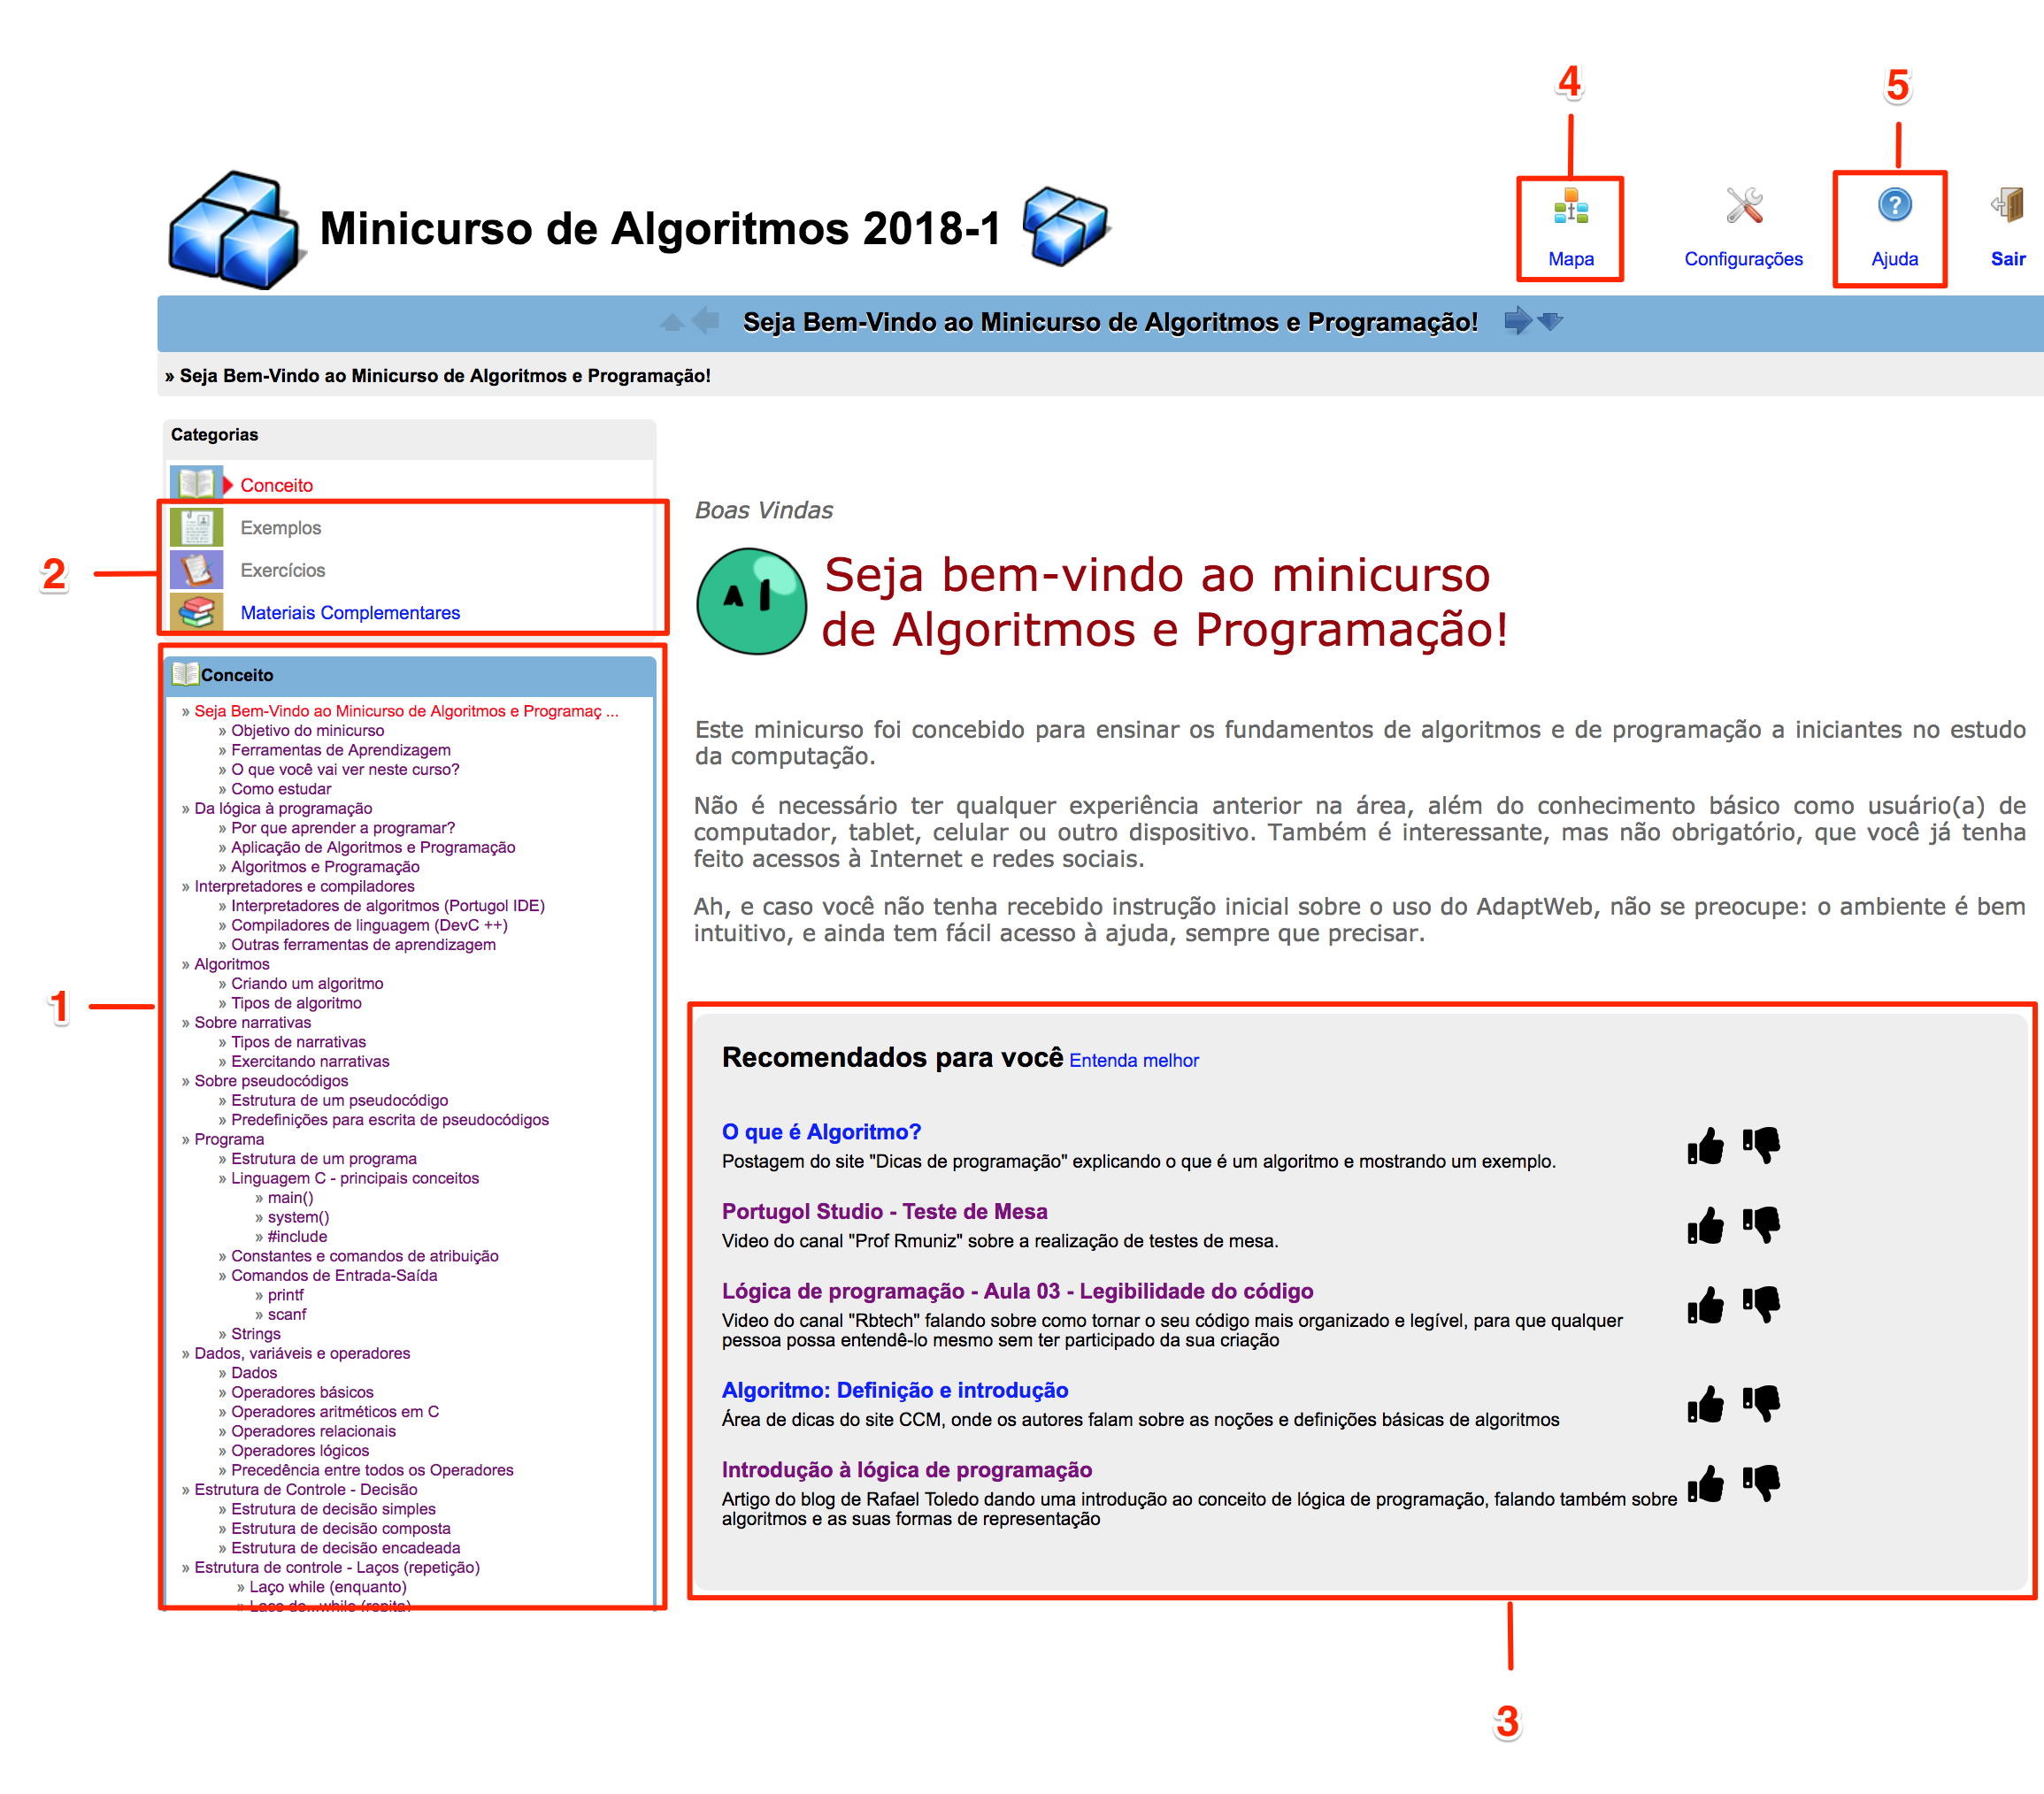
\includegraphics[scale=0.4]{./Figuras/interface-recomendacao.png}
  \end{center}
  \legend{Fonte: O autor.}
\end{figure}

Como visto na imagem, as principais informações dos Links de Apoio apresentadas para o aluno são: Link, Nome do Link,
Descrição e a possibilidade de avaliar o item positivamente ou negativamente. A avaliação feita pelo usuário não é
considerada pelo algoritmo de recomendação, sendo que os itens acessados pelo
usuário são considerados como do seu interesse. Como trabalho futuro é possível incorporar a avaliação na recomendação, e.g.,
não tornar a recomendar itens que foram avaliado com notas baixas ou apenas considerar para o algoritmo Baseado em Conteúdo
os itens avaliados positivamente. \citeonline{pu2012evaluating} afirmam que enquanto recomendar um item apenas é pouco, recomendar mais do que cinco itens
aumenta a dificuldade de escolhar do usuário. Por isso, a quantidade máxima de itens recomendadas para o usuário em cada
recomendação é de cinco itens.

Para cumprir o requisito de Explicação das recomendações citada por \citeonline{pu2012evaluating}, foi adicionado o
botão de ''Entenda melhor'' que tem por objetivo explicar ao usuário como a lista de itens foi gerada. Ao entender o
funcionamento do algoritmo de recomendação, o usuário tem a possibilidade aprimorar o seu perfil para personalizar as
recomendações recebidas. Na Figura \ref{fig:adaptweb-proposta-explicacao} está a explicação das recomendações
mostrada para o aluno.

\begin{figure}[htb]
  \caption{\label{fig:adaptweb-proposta-explicacao}Explicação da recomendação}
  \begin{center}
      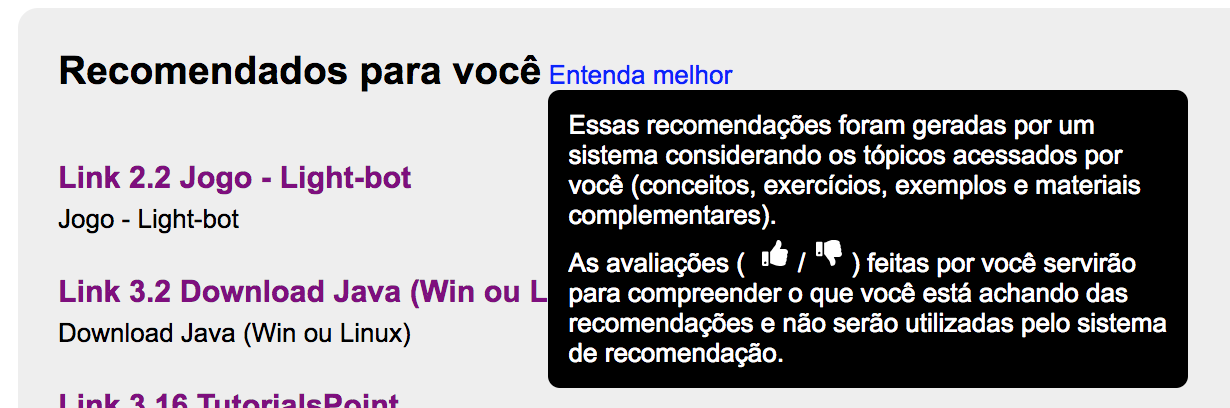
\includegraphics[scale=0.6]{./Figuras/explicacao-das-recomendacoes.png}
  \end{center}
  \legend{Fonte: O autor.}
\end{figure}

\subsection{Definição do experimento}\label{subsection:definicao-experimento}

Para a execução do experimento, o SR proposto foi comparado a abordagem Baseada em Conteúdo tradicional utilizando uma
estratégia \textit{Between Subjects}, i.e., os alunos foram divididos em dois grupos e cada grupo utilizou apenas
um dos sistemas. Para garantir que a única variável seja o SR utilizado, ambos os grupos utilizaram a mesma
interface proposta para as recomendações.

O experimento proposto neste trabalho visa avaliar o desempenho e a percepção do usuário do SR proposto quando
comparado à abordagem Baseada em Conteúdo Tradicional. Para avaliar o desempenho do algoritmo de recomendação em relação
à variável independente \textit{Algoritmo de Recomendação} foram adotadas as seguintes hipóteses:

\begin{itemize}
\item \textbf{H\textsubscript{0}:} Não há diferenças entre o desempenho da abordagem Baseada em Conteúdo
Tradicional e a proposta desse trabalho.
\item \textbf{H\textsubscript{1}:} Há diferenças entre o desempenho da abordagem Baseada em Conteúdo
Tradicional e a proposta desse trabalho.
\end{itemize}

Para avaliar a percepção do usuário sobre a qualidades das recomendações recebidas em relação
à variável independente \textit{Algoritmo de Recomendação} foram adotadas as seguintes hipóteses:

\begin{itemize}
\item \textbf{H\textsubscript{0}:} Não há diferenças na percepção do usuário da qualidade das recomendações recebidas utilizando a abordagem
Baseada em Conteúdo tradicional e a proposta desse trabalho.
\item \textbf{H\textsubscript{1}:} Há diferenças na percepção do usuário da qualidade das recomendações recebidas utilizando a abordagem
Baseada em Conteúdo tradicional e a proposta desse trabalho.
\end{itemize}

O experimento foi realizado através do Minicurso de Algoritmos e Linguagem de Programação, o qual teve seu design
instrucional realizado por \citeonline{santos2017addie}. Foram convidados a participar alunos dos cursos do
Centro de Ciências Tecnológicas (CCT) da Universidade do Estado de Santa Catarina (UDESC) que possuem essa disciplina na
grade curricular, i.e.: Bacharelado em Ciência da Computação, Tecnólogo em Análise e Desenvolvimento de Sistemas, Engenharia
Elétrica, Engenharia Civil, Engenheria Mecânica, Engenharia da Produção, Matemática e Física. Os convites foram
realizados diretamente nas salas das disciplinas de Algoritmos, Algoritmos e Linguagem de Programação, Linguagem de
Programação e Iniciação a Ciência da Computação. Além disso, foi enviado um convite para todos os alunos do campus por
e-mail através da Assessoria de Comunicação e foi divulgado na página do Facebook da UDESC Joinville.

Os usuários que se matricularam no Minicurso foram aleatoriamente divididos em dois grupos, da forma mais igualitária possível
pelos seguintes critérios: Professor, Curso, Sexo e Idade. Isso foi possível
porque durante o processo de matrícula os alunos responderam um questionário para montar o seu perfil. Também durante a
matrícula os alunos tiveram acesso ao Termo de Consentimento Livre e Esclarecido, presente no Apêndice
\ref{ape:termo-de-consentimento}, que explica o objetivo do experimento e no qual eles consentiram em participar e em
permitir o uso dos resultados para essa pesquisa, garantindo a anonimidade dos participantes.

Ao final do minicurso, os alunos puderam acessar a avaliação do Minicurso, composta de 10 questões, e o questionário
sobre a percepção do usuário sobre o SR. As questões do questionário foram selecionadas de um
conjunto de questões definidas por \citeonline{pu2011user} (presente no Anexo \ref{ane:questoes-framework}), considerando
um dos objetivos desse experimento que é medir a percepção do usuário sobre as recomendações recebidas.
As questões selecionadas foram traduzidas para o Português e estão presentes no Apêndice \ref{ape:questionario-de-satisfacao}.
Além dessas questões, foi adicionada uma questão discursiva perguntando sobre os pontos positivos e negativos do SR utilizado.

Durante o desenvolvimento do Minicurso foram utilizadas as Intervenções definidas por \citeonline{santos2017addie}, para
fazer com que os alunos fiquem engajados no curso. As Intervenções são e-mails combinadas com postagens no Fórum de Discussão
que guiam os alunos no seu estudo e também propõe desafios para os estudantes. As Intervenções propostas por \citeonline{santos2017addie}
consideram o Minicurso com uma duração de dois meses, por isso foi necessário uma adaptação dessas Intervenções para o período
mais reduzido no qual foi realizado esse experimento. As Intervenções de \citeonline{santos2017addie}, com as adaptações
necessárias como data de início do experimento, podem
ser vistar no Anexo \ref{ane:intervencoes} e os Desafios postados no Fórum de Discussão estão presentes no Apêndice \ref{ane:desafios}.

\subsection{Teste piloto}\label{section:planejamento-teste-piloto}

Antes do experimento ser realizado com os alunos no Minicurso de Algoritmos, foi realizado um teste piloto com
quatro alunos que já realizaram essa disciplina. O objetivo do teste piloto foi avaliar os instrumentos do experimento,
além de permitir encontrar problemas na experiência do usuário para serem corrigidos antes da execução do minicurso. O teste piloto
foi realizado no dia 06 de Abril de 2018.

Durante o teste piloto os alunos foram divididos em dois grupos aleatóriamente, sendo que dois alunos utilizaram o SR
Baseado em Conteúdo Tradicional e os outros dois utilizaram o SR com o Decaimento. Os alunos receberam
um protocolo de atividades para realizar, presente no Apêndice \ref{ape:teste-piloto}. As tarefas envolvem
realizar a matrícula na disciplina, na qual eles leram e aceitaram o Termo de Consentimento Livre e Esclarecido, realizar
o acesso a alguns conceitos e materiais complementares, utilizar o SR, realizar a avaliação da disciplina e responder
ao questionário sobre a experiência com o SR. Durante o teste, os comentários e observações feitas pelos alunos foram
anotadas para posterior análise.

Os quatro participantes do teste piloto foram identificados como Participante 1, Participante 2,
Participante 3 e Participante 4. Os Partipantes 1 e 2 utilizaram o algoritmo tradicional de recomendação, enquanto os
participantes 3 e 4 utilizaram a proposta desse trabalho, porém eles não sabiam disso durante a realização do Teste. Os
participantes foram livres na escolha do Sistema Operacional e Navegador utilizados, bem como no Modo de Navegação
escolhido (Livre ou Tutorial). A Tabela \ref{tab:participantes-teste-piloto} apresenta o Modo de Navegação e o Algoritmo
de Recomendação utilizado por cada participante.

\begin{table}[h]
\footnotesize
\caption[Dados dos Participantes do Teste Piloto]{Dados dos Participantes do Teste Piloto}
\label{tab:participantes-teste-piloto}
\centering
\begin{tabular}{|p{2cm}|p{3.5cm}|p{6.5cm}|}
  \hline
  \textbf{Participante} & \textbf{Modo de Navegação} & \textbf{Algoritmo de Recomendação} \\
  \hline
  1 & Tutorial & Baseado Em Conteúdo Tradicional \\
  \hline
  2 & Livre & Baseado Em Conteúdo Tradicional \\
  \hline
  3 & Tutorial & Baseado Em Conteúdo com Decaimento \\
  \hline
  4 & Livre & Baseado Em Conteúdo com Decaimento \\
  \hline
\end{tabular}
\legend{Fonte: O autor.}
\end{table}

Durante a execução do Teste Piloto, os participantes encontraram erros de digitação no Termo de Consentimento Livre e Esclarecido (TCLE)
e alguns problemas na prova da disciplina, como perguntas de Verdadeiro e Falso com questões duplicadas e uma
pergunta que não possuía nenhuma resposta certa. Esses problemas foram todos resolvidos antes do início do experimento.

Sobre as recomendações, os Participantes 1 e 2 comentaram que que as recomendações recebidas eram quase sempre as mesmas,
mesmo tendo acessado conceitos diferentes - mudando apenas de ordem. Já os Participantes
3 e 4, que utilizaram a proposta desse trabalho, comentaram que ao acessar um novo conceito pelo menos 3 novos Links eram
recomendados. Essa observação dos participantes demonstra o problema da Superespecilização presente na Abordagem Baseada
em Conteúdo Tradicional, e mostra que a proposta desse trabalho utilizando o Decaimento ajuda a diminuir esse problema.

Os participantes também observaram que desde o primeiro acesso a disciplina eles receberam cinco links com recomendação, i.e.,
o número máximo possível. Isso mostra que, como não foi definido um limiar mínimo para a similaridade entre o perfil do usuário
e os Links de Apoio, mesmo que a similaridade seja muito pequena o algoritmo sempre irá recomendar algo para o aluno. Por
outro lado, não seria interessante adicionar um limiar para o experimento deste trabalho pois estaria adicionando
mais uma variável independente ao experimento. Como trabalho futuro é possível analisar como o limiar mínimo para a
similaridade pode afetar a qualidade percebida das recomendações.

Ao final do Teste Piloto foi realizada uma pequena entrevista com os participantes onde eles afirmaram ter entendido
a interface do SR. Quando revelado que cada participante existiam dois SRs e que duas pessoas estavam usando a abordagem
Tradicional e os outros dois estavam usando a proposta do trabalho, os participantes associaram essa informação com os
comentários que feitos sobre da Superespecialização, pelos alunos da abordagem Tradicional, e a novidade nas recomendações,
pelos alunos da Proposta.

\section{Execução}\label{section:execucao-experimento}

O período de matrícula para o minicurso foi de 09 de Abril de 2018 até 13 de Abril de 2018. Durante esse período, todas
as turmas das disciplinas mencionadas na Seção \ref{subsection:definicao-experimento} foram visitadas, convidando os
alunos a se matricular no minicurso. O apoio dos professores das disciplinas foi essencial nessa etapa.

No total, 208 alunos se matricularam no Minicurso. Esses alunos foram homogeneamente divididos em dois grupos
(AlgoritmoTradicional e AlgoritmoProposta) utilizando os seguintes critérios: Professor, Curso, Sexo e Idade. A
Tabela \ref{tab:divisao-alunos-experimento} mostra o resultado da divisão dos alunos.

\begin{table}[h]
\footnotesize
\caption[Divisão dos alunos de acordo com os critérios]{Divisão dos alunos de acordo com os critérios}
\label{tab:divisao-alunos-experimento}
\centering
\begin{tabular}{|c|c|c|c|c|}
  \hline
  \multicolumn{3}{|c|}{}                                                                         & \multicolumn{2}{c|}{\textbf{Algoritmo de Recomendação}} \\ \hline
  \multicolumn{2}{|c|}{\textbf{Critério}}                  & \multicolumn{1}{c|}{\textbf{Total}} & AlgoritmoTradicional & AlgoritmoProposta                \\ \hline
  \multirow{12}{*}{Professor}           & Professor A      & 12                                  & 6                    & 6                                \\
                                        & Professor B      & 18                                  & 9                    & 9                                \\
                                        & Professor C      & 7                                   & 4                    & 3                                \\
                                        & Professor D      & 5                                   & 3                    & 2                                \\
                                        & Professor E      & 38                                  & 19                   & 19                               \\
                                        & Professor F      & 4                                   & 2                    & 2                                \\
                                        & Professor G      & 10                                  & 5                    & 5                                \\
                                        & Professor H      & 6                                   & 3                    & 3                                \\
                                        & Professor I      & 6                                   & 3                    & 3                                \\
                                        & Professor J      & 26                                  & 13                   & 13                               \\
                                        & Professor K      & 14                                  & 7                    & 7                                \\
                                        & Outro            & 52                                  & 30                   & 32                               \\ \hline
  \multirow{9}{*}{Curso}                & Computação       & 55                                  & 23                   & 22                               \\
                                        & TADS             & 36                                  & 18                   & 18                               \\
                                        & Elétrica         & 36                                  & 18                   & 18                               \\
                                        & Física           & 10                                  & 5                    & 5                                \\
                                        & Mecânica         & 31                                  & 15                   & 16                               \\
                                        & Química          & 3                                   & 2                    & 1                                \\
                                        & Produção         & 20                                  & 10                   & 10                               \\
                                        & Civil            & 15                                  & 7                    & 8                                \\
                                        & Matematica       & 12                                  & 6                    & 6                                \\ \hline
  \multirow{3}{*}{Sexo}                 & Masculino        & 135                                 & 67                   & 68                               \\
                                        & Feminino         & 72                                  & 36                   & 36                               \\
                                        & Não informado    & 1                                   & 1                    & 0                                \\ \hline
  \multirow{6}{*}{Idade}                & Até 17 anos      & 21                                  & 10                   & 11                               \\
                                        & 18 ou 19 anos    & 75                                  & 37                   & 38                               \\
                                        & 20 ou 21 anos    & 35                                  & 18                   & 17                               \\
                                        & 22 ou 23 anos    & 11                                  & 6                    & 5                                \\
                                        & 24 ou 25 anos    & 26                                  & 13                   & 13                               \\
                                        & 26 anos ou mais  & 40                                  & 20                   & 20                               \\ \hline
                                        & Total            & 208                                 & 104                  & 104                              \\ \hline
\end{tabular}
\end{table}

O período de execução do Minicurso foi de 16 de Abril de 2018 até 10 de Maio de 2018. Nesse período, dos 208 alunos
matriculados no Minicurso, 145 acessaram a disciplina pelo menos uma vez, sendo 76 do grupo AlgoritmoTradicional e 69
do grupo AlgoritmoProposta.

O período para realizar a prova da disciplina e responder ao questionário foi de 11 de Maio de 2018 até
14 de Maio de 2018. Nesse período, dos 145 alunos que acessaram a disciplina pelo menos uma vez, 85 realizaram a prova final e responderam ao
questionário, sendo 48 do grupo AlgoritmoTradicional e 37 do grupo AlgoritmoProposta. Dos 85 alunos que finalizaram a
disciplina (i.e., realizaram a prova e responderam ao questionário), 47 acessaram pelo menos uma recomendação que
recebeu, sendo 25 do grupo AlgoritmoTradicional e 22 do grupo AlgoritmoProposta. A Tabela \ref{tab:uso-minicurso-sr}
apresenta mais informações sobre as ações dos alunos dentro do \adaptweb.

\begin{table}[h]
\footnotesize
\centering
\caption{Uso do Minicurso de Algoritmos e do SR}
\label{tab:uso-minicurso-sr}
\begin{tabular}{|p{9.5cm}|p{2cm}|p{1.5cm}|p{1cm}|}
\hline
\textbf{Quantidade de:}                                                                     & \textbf{Tradicional} & \textbf{Proposta}    & \textbf{Total}    \\
\hline
Alunos que se matricularam                                                                  & 104                  & 104                  & 208      \\
\hline
Alunos que entraram pelo menos uma vez no curso                                             & 76                   & 69                   & 145      \\
\hline
Alunos que acessaram pelo menos uma recomendação                                            & 46                   & 39                   & 85       \\
\hline
Alunos que avaliaram pelo menos uma recomendação                                            & 30                   & 22                   & 52       \\
\hline
Alunos que realizaram a prova                                                          & 48                   & 38                   & 86       \\
\hline
Alunos que responderam o questionário                                         & 48                   & 37                   & 85       \\
\hline
Alunos que responderam o questionário e acessaram pelo menos uma recomendação & 25                   & 22                   & 47       \\
\hline
Alunos que responderam o questionário e avaliaram pelo menos uma recomendação & 16                   & 13                   & 29       \\
\hline
Acessos aos itens recomendados                                                              & 227                  & 396                  & 623      \\
\hline
Avaliações positivas ao itens recomendados                                                  & 141                  & 234                  & 375      \\
\hline
Avaliações negativas ao itens recomendados                                                  & 5                    & 4                    & 9        \\
\hline
\end{tabular}
\end{table}

Pela Tabela \ref{tab:uso-minicurso-sr} podemos perceber que 38 alunos que responderam ao questionário não acessaram nenhuma
recomendação, sendo 23 do grupo AlgoritmoTradicional e 15 do grupo AlgoritmoProposta. Na Seção
\ref{subsection:analise-uso-sr} os dados de acesso e avaliação das recomendações são analisadas mais profundamente,
comparando os resultados dos dois algoritmos utilizando técnicas estatísticas descritas na Seção \ref{subsection:tecnicas-analise-estatistica}.

\section{Análise dos Resultados}\label{section:analise-experimento}

Nessa seção são descritas as análises estatísticas realizadas sobre os dados coletados durante a execução do experimento.
As técnicas estatísticas utilizadas para fazer a análise são apresentadas na Seção \ref{subsection:tecnicas-analise-estatistica}
e nas Subseções subsequentes são apresentas as análises realizadas sobre o desempenho dos algoritmos de recomendação e sobre
a percepção dos alunos sobre a qualidade do SR utilizado.

\subsection{Técnicas de Análise Estatística}\label{subsection:tecnicas-analise-estatistica}

Para realizar as análises estatísticas, primeiro foi necessário entender os tipos de variáveis que podem ser analisadas.
As variáveis são as informações coletadas durante o experimento e podem ser quantitativas ou qualitativas \cite{bussab2012morettin}.
As variváveis quantitativas são resultado de uma contagem e/ou mensuração \cite{bussab2012morettin} e podem ser discretas
(conjunto finito ou enumerável de números) ou contínuas (pertencem a um intervalo de números reais). Exemplos de variáveis
quantitativas são número de filhos, número de cômodos em uma casa, número de pessoas presentes em uma sala, altura e peso.
As variáveis qualitativas são aquelas que descrevem um aspecto relacionado ao objeto estudado \cite{bussab2012morettin} e podem ser
nominais (quando não possuem ordenação) ou ordinais (quando há ordem entre os valores). Exemplos de variáveis qualitativas
são sexo, estado civil e grau de instrução.

A variável independente desse trabalho é o algoritmo de recomendação utilizado pelo alunos, que pode assumir os valores
AlgoritmoTradicional ou AlgoritmoProposta. As variáveis dependentes analisadas são o
desempenho do algoritmo de recomendação e a percepção do usuário sobre as recomendações. O desempenho do SR
foi medido através da quantidade de recomendações acessadas, quantidade de recomendações avaliadas, Precisão e Cobertura do
algoritmo. A quantidade de recomendações acessadas e/ou avaliadas são variáveis quantitativas discretas,
enquanto a Precisão e a Cobertura do algoritmo de recomendação são variáveis quantitativas contínuas. A percepção do usuário sobre
as recomendações recebidas, que foi medida através do questionário, pode ser categorizado como uma variável
qualitativa ordinal, pois as respostas da escala de Likert podem ser ordenadas de Discordo Totalmente até Concordo Totalmente.

De acordo com o tipo de variável analisado e a distribuição dos valores dessa variável é possível definir qual técnica
estatística será utilizada. O fluxograma da Figura \ref{fig:fluxograma-tecnica-moissa} produzido por \citeonline{moissa2016influencia}
define como decidir as técnicas estatísticas utilizadas. Todos os testes mencionados na Figura \ref{fig:fluxograma-tecnica-moissa}
estão disponíveis na ferramenta estatística R \cite{rstatisticalcomputing2018}, que foi a ferramenta utilizada para todas as análises realizadas nas
Subseções a seguir.

\begin{figure}[htb]
  \caption{\label{fig:fluxograma-tecnica-moissa}Fluxograma de uso das técnicas estatísticas}
  \begin{center}
      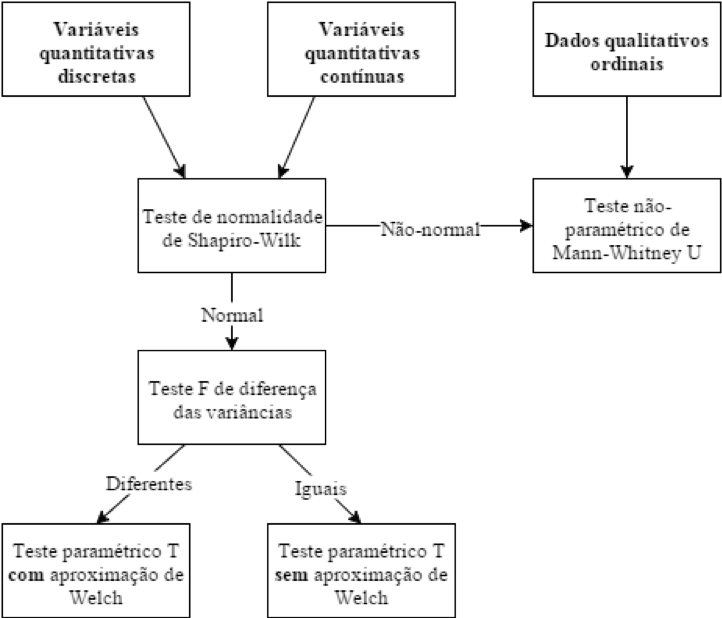
\includegraphics[scale=1.0]{./Figuras/fluxograma-tecnicas-moissa.png}
  \end{center}
  \legend{Fonte: \citeonline{moissa2016influencia}}
\end{figure}

\subsection{Análise do Desempenho da Abordagem de Recomendação}\label{subsection:analise-uso-sr}

Nessa seção é realizada uma análise estatística sobre os acessos e avaliações dos usuários aos Links de Apoio recomendados.
O objetivo é extrair informações dos dados capturados durante a interação para avaliar o desempenho do algoritmo em
relação a diversas métricas. As análises feitas foram da (1) Quantidade de recomendações acessadas,
(2) Quantidade de avaliações positivas para as recomendações, (3) Quantidade de avaliações negativas para as recomendações,
(4) Precisão do algoritmo de recomendação, (5) Cobertura do algoritmo de recomendação e (6) F-measure do algoritmo de
recomendação, comparando os alunos que utilizaram a abordagem Baseada em Conteúdo Tradicional com os alunos
que utilizaram a Proposta desse trabalho. Os resultados das análises realizadas nessa Seção estão presentes no Apêndice \ref{ape:analise-estatistica-do-uso}.

Para a análise da quantidade de recomendações acessadas, foram considerados apenas os alunos que acessaram pelo
menos uma recomendação no ambiente (i.e., 85 alunos). A média do grupo AlgoritmoTradicional foi de 4,935 itens
acessados por aluno, enquanto no grupo AlgoritmoProposta foi de 6,5 itens. A análise utilizando o Teste de normalidade de
Shapiro-Wilk mostrou que a distribuição dos dados não é normal e portanto o Teste não-paramétrico de Mann-Whitney U foi utilizado
para comparar os dois fatores. Esse Teste mostrou que não existe diferença significativa entre as amostras e portanto
não podemos que afirmar que existe diferença na quantidade de recomendações acessadas nos dois grupos analisados.

A análise realizada sobre as avaliações positivas para as recomendações utilizou apenas os alunos que avaliaram positivamente
alguma recomendação (i.e., 52 alunos). A média da quantidade de avaliações positivas para o grupo AlgoritmoTradicional
foi de 4,7 avaliações por aluno, enquanto no grupo AlgoritmoProposta foi de 10,64 avaliações por aluno.
Essa análise teve um resultado similar ao anterior, onde o Teste de normalidade de Shapiro-Wilk também mostrou que a
distribuição é não-normal e o Teste de Mann-Whitney U mostrou que não existem diferença signifitiva entre
as amostras dos dois grupos.

A análise da quantidade de avaliações negativas para as recomendações utilizou apenas os alunos que avaliaram negativamente
os itens (i.e., 7 alunos). A média de avaliações para o grupo que AlgoritmoTradicional foi de 1 avaliação negativa
por aluno, enquanto para o grupo AlgoritmoProposta foi de 2 avaliações negativas por aluno. Ao realizar
a análise estatística, o Teste de normalidade de Shapiro-Wilk mostrou que a distribuição dos dados é não-normal. O Teste
não-paramétrico de Mann-Whitney U foi aplicado e mostrou que não existe diferença significativa para esse critério entre
os dois grupos.

A Precisão dos algoritmos de recomendação foi calculada para cada aluno que acessou pelo menos uma recomendação dentro do
ambiente (i.e., 85 alunos) dividindo a quantidade de recomendações distintas acessadas pelo usuário pela quantidade de
itens distintos que foram recomendados para o usuário durante todo o minicurso. Essa métrica resulta em um valor entre
0 e 1, onde um valor próximo de 0 indica que poucos dos itens recomendados foram acessados e um valor próximo de 1
mostra que a maioria dos itens recomendados foram acessados, independente da quantidade de vezes que um item foi
acessado e da quantidade de vezes que o item foi recomendado. A média da Precisão para o grupo AlgoritmoTradicional foi
0,49679 e para o AlgoritmoProposta foi 0,39859. O Teste de normalidade de Shapiro-Wilk mostra que a distruibuição dos
dados da Precisão é não-normal e o Teste de Mann-Whitney U mostrou que não existem diferença signifitiva entre as
precisão calculada para cada algoritmo.

A Cobertura dos algoritmos da recomendação foi calculada considerando os alunos que acessaram pelo menos uma recomendação
dentro do Minicurso (i.e., 85 alunos). Essa métrica foi calculada dividindo a quantidade de itens distintos recebidos
como recomendação pelo usuário pela quantidade de itens disponíveis para recomendação na disciplina (i.e., 108 itens) e mostra
a porcentagem dos itens disponíveis para recomendação que foram efetivamente recomendados. A média da Cobertura para o
grupo AlgoritmoTradicional é de 0,10064 e para o AlgoritmoProposta é de 0,17450. Ao realizar o Teste de
normalidade de Shapiro-Wilk o resultado mostrou que a distribuição dos dados é não-normal. Quando aplicado o Teste de Mann-Whitney
U o resultado mostrou que existe diferença significativa entre os resultados dos dois grupos com relação à Cobertura e, nesse caso,
podemos afirmar que o algoritmo Com Decaimento tem uma Cobertura melhor que a algoritmo Tradicional. Essa diferença significativa
mostra que a Proposta desse trabalho ajuda a diminuir o problema da Superespecialização presente na abordagem Tradicional.

Como visto na Seção \ref{section:fundamentacao-avaliacao-sr}, o \textit{F-measure} é calculado como a média harmônica entre
a Precisão e o \textit{Recall} do algoritmo. Essa métrica é interessante para garantir que o algoritmo não diminua o \textit{Recall}
para aumentar a Precisão, e vice-versa. Como no experimento realizado o \textit{Recall} não pode ser determinado, pois não
é possível saber todos os itens relevantes existentes para cada usuário (essa métrica é mais comum em experimentos
\textit{offline}), nesse trabalho foi utilizado a Cobertura no cálculo do \textit{F-measure} ao invés do \textit{Recall}.
Com isso podemos mostrar se o algoritmo Proposto teve uma melhor Cobertura que a abordagem Tradicional sem diminuir
a sua Precisão. A análise foi realizada utilizando os 85 alunos que acessaram pelo menos uma recomendação e o valor médio
dessa métrica proposta foi de 0,13852 para o grupo AlgoritmoTradicional e de 0,21719 o grupo AlgoritmoProposta.
O Teste de Normalidade de Shapiro-Wilk mostrou que a distribuição dos dados é não-normal e portanto o Teste de
Mann-Whitney U foi utilizado para verificar a diferença significativa entre os dois grupos. Esse teste mostrou que
existe diferença significativa entre os dois grupos e portanto podemos afirmar que F-measure, com a Cobertura ao invés
do \textit{Recall}, teve um resultado melhor para o algoritmo proposto do que na abordagem tradicional. Isso mostra
que o uso do Decaimento aumentou a Cobertura do algoritmo sem influenciar negativamente outros aspectos, como a Precisão.

Como a Cobertura e F-measure deram diferença significativa, podemos aceitar a hipótese alternativa definida
que diz que ''Há diferenças entre o desempenho da abordagem Baseada em Conteúdo Tradicional e a proposta desse trabalho''
e a diferença significativa nos dois casos foi favorável a proposta desse trabalho.

\subsection{Análise da Percepção do Usuário}\label{subsection:analise-questionario-satisfacao}

A percepção dos usuários da qualidade das recomendações recebidas foi medida por meio do questionário presente no
Apêndice \ref{ape:questionario-de-satisfacao}. O questionário possui 13 questões que foram selecionadas do questionário
definido por \citeonline{pu2011user} (presente no Anexo \ref{ane:questoes-framework}) e traduzidas para o Português.
Essas questões são afirmações nas quais os alunos devem se posicionar em uma escala de
Likert de cinco pontos, de ''Discordo Totalmente'' até ''Concordo Totalmente''. Também foi adicionada uma opção de ''Não utilizei'' para
os alunos que não utilizaram o SR (ou usaram sem perceber). A Tabela \ref{tab:questionario-satisfacao-respostas}
apresenta as respostas agrupadas dos alunos para cada uma das perguntas.

\begin{table}[h]
\footnotesize
\caption{Respostas ao Questionário}
\label{tab:questionario-satisfacao-respostas}
\centering
\begin{tabular}{|p{1.5cm}|p{1.8cm}|p{2.2cm}|p{0.6cm}|p{0.6cm}|p{0.6cm}|p{2.3cm}|p{2cm}|}
\hline
\textbf{Questão} & \textbf{Algoritmo}   & \textbf{Discordo tot.} & \textbf{-} & \textbf{-} & \textbf{-} & \textbf{Concordo tot.} & \textbf{Não utilizei} \\
\hline
\multirow{2}{*}{1}          & Tradicional & 2                   & 1                     & 2                         & 15                    & 11                  & 17           \\
                            & Proposta    & 0                   & 0                     & 6                         & 11                    & 7                   & 13           \\
\hline
\multirow{2}{*}{2}          & Tradicional & 1                   & 0                     & 5                         & 18                    & 6                   & 18           \\
                            & Proposta    & 0                   & 1                     & 7                         & 9                     & 9                   & 11           \\
\hline
\multirow{2}{*}{3}          & Tradicional & 2                   & 0                     & 8                         & 13                    & 8                   & 17           \\
                            & Proposta    & 0                   & 2                     & 4                         & 12                    & 8                   & 11           \\
\hline
\multirow{2}{*}{4}          & Tradicional & 1                   & 0                     & 5                         & 17                    & 6                   & 19           \\
                            & Proposta    & 0                   & 1                     & 8                         & 8                     & 10                  & 10           \\
\hline
\multirow{2}{*}{5}          & Tradicional & 3                   & 0                     & 4                         & 10                    & 10                  & 21           \\
                            & Proposta    & 0                   & 2                     & 9                         & 8                     & 6                   & 12           \\
\hline
\multirow{2}{*}{6}          & Tradicional & 3                   & 3                     & 3                         & 12                    & 8                   & 19           \\
                            & Proposta    & 0                   & 0                     & 5                         & 11                    & 10                  & 11           \\
\hline
\multirow{2}{*}{7}          & Tradicional & 2                   & 5                     & 4                         & 14                    & 9                   & 14           \\
                            & Proposta    & 1                   & 1                     & 7                         & 9                     & 7                   & 12           \\
\hline
\multirow{2}{*}{8}          & Tradicional & 0                   & 6                     & 3                         & 12                    & 9                   & 18           \\
                            & Proposta    & 0                   & 2                     & 8                         & 8                     & 6                   & 13           \\
\hline
\multirow{2}{*}{9}          & Tradicional & 2                   & 2                     & 7                         & 10                    & 7                   & 20           \\
                            & Proposta    & 0                   & 0                     & 11                        & 5                     & 8                   & 13           \\
\hline
\multirow{2}{*}{10}         & Tradicional & 1                   & 0                     & 10                        & 14                    & 4                   & 19           \\
                            & Proposta    & 0                   & 2                     & 4                         & 12                    & 8                   & 11           \\
\hline
\multirow{2}{*}{11}         & Tradicional & 2                   & 2                     & 6                         & 13                    & 5                   & 20           \\
                            & Proposta    & 0                   & 1                     & 6                         & 10                    & 8                   & 12           \\
\hline
\multirow{2}{*}{12}         & Tradicional & 4                   & 1                     & 6                         & 17                    & 2                   & 18           \\
                            & Proposta    & 0                   & 1                     & 5                         & 9                     & 10                  & 12           \\
\hline
\multirow{2}{*}{13}         & Tradicional & 2                   & 0                     & 6                         & 13                    & 12                  & 15           \\
                            & Proposta    & 0                   & 1                     & 4                         & 7                     & 14                  & 11           \\
\hline
\end{tabular}
\end{table}

Através das respostas dos alunos presentes na Tabela \ref{tab:questionario-satisfacao-respostas}, podemos perceber que
o grupo AlgoritmoTradicional tem mais respostas de ''Discordo Totalmente'' do
que o grupo AlgoritmoProposta, com 25 para o AlgoritmoTradicional e uma para o AlgoritmoProposta.
Além disso, pode-se perceber que 12 questões tiveram pelo menos um ''Discordo Totalmente'' para o grupo AlgoritmoTradicional
e uma questão para o grupo AlgoritmoProposta. Com relação a resposta ''Concordo Totalmente'',
97 respostas foram dadas pelos alunos do grupo AlgoritmoTradicional e 111
pelos alunos do grupo AlgoritmoProposta. Por outro lado, tiveram mais respostas ''Discordo Parcialmente'',
''Não Concordo e Nem Discordo'' e ''Concordo Parcialmente'' para o grupo AlgoritmoTradicional do que para o grupo
AlgoritmoProposta, com 267 para o primeiro e 217 para o segundo.

O resultado das respostas ''Não utilizei'' mostram que os alunos responderam que não utilizaram para apenas algumas
perguntas e não para todas, sendo que para o grupo AlgoritmoTradicional o valor varia entre 17 e 21 alunos e para o grupo
AlgoritmoProposta varia entre 10 e 13 alunos. O fato desse valor ter variado tanto não foi esperado inicialmente, mas pode-se
afirmar que pelo menos 17 alunos do primeiro grupo e 10 alunos do segundo grupo não utilizaram o SR. Ao comparar essa
informação com os dados de acesso dos alunos, que mostra que 23 alunos do grupo AlgoritmoTradicional e 15 alunos do
grupo AlgoritmoProposta não acessaram nenhuma recomendação, é provável que apesar de não terem acessado nenhuma recomendação os
alunos perceberam a existência do SR, analisaram as recomendações recebidas e com base nisso responderam às questões do
questionário.

As respostas dadas ao questionário foram analisadas utilizando o Teste não-paramétrico de
Mann-Whitney U para verificar se existe diferença estatisticamente significativa entre as respostas dos dois grupos (i.e., \textit{p} < 0.05).
As respostas de ''Não utilizei'' não foram consideradas nessa análise. O resultado das análises está presente no Apêndice
\ref{ape:analise-estatistica-questionario}.

A análise mostrou que a questão 12 (i.e., ''Eu entendi porque os itens foram recomendados para mim.'') apresentou
diferença significativa entre as respostas dos dois grupos, e a diferença foi favorável ao grupo AlgoritmoProposta.
Para as outras questões não foi encontrada diferença significativa entre as respostas dos
alunos dos dois grupos. A diferença existente na questão 12 mostra que os alunos do grupo AlgoritmoProposta perceberam
melhor a relação entre os conteúdos que acessaram com os links que foram recomendados para eles
do que o grupo AlgoritmoTradicional. Essa informação mostra que o uso do Decaimento na Abordagem
Baseada em Conteúdo fez com que as recomendações geradas fossem relacionadas aos conteúdos acessados recentemente,
enquanto a Abordagem Tradicional recomenda considerando todos os conteúdos acessados pelo aluno durante todo o Minicurso
igualmente.

Como pelo menos uma questão do questionário deu diferença significativa, podemos aceitar a hipótese alternativa definida
que diz que ''Há diferenças na percepção do usuário da qualidade das recomendações recebidas utilizando a abordagem
Baseada em Conteúdo tradicional e a proposta desse trabalho'' e a diferença significativa foi favorável a proposta desse trabalho.

\subsection{Questão Discursiva sobre o SR}\label{subsection:questao-aberta}

Juntamente com o questionário de satisfação, foi colocada um questão discursiva para alunos com a seguinte pergunta:
''Você utilizou o Sistema de Recomendação? Se sim, cite os pontos positivos e negativos desse sistema.''. Dos 85 alunos
que responderam à essa questão, 60 disseram não ter utilizado ou ter utilizado muito pouco o SR
e não citaram nenhum ponto positivo ou negativo, sendo 36 do grupo AlgoritmoTradicional
e 24 do grupo AlgoritmoProposta. Dois alunos do grupo AbordagemTradicional disseram
não ter utilizado o SR pois não perceberam a sua existência e um aluno desse mesmo grupo disse que não utilizou com tanta frequência
pois não entendeu como este funcionava. Um aluno do grupo AlgoritmoProposta disse não ter utilizado
o SR pois achou que o conteúdo do Minicurso de Algoritmos era bem completo e não viu necessidade de acessar as recomendações.

Os pontos positivos e negativos apontados pelos alunos que utilizaram o SR foram analisados utilizando a técnica de análise
e interpretação de dados qualitativos como descrito por \citeonline{creswell2014research}. O processo de análise e interpretação
é composto pelos seguintes passos: (1) Organizar e preparar os dados para análise;
(2) Ler todos os dados; (3) Codificar os dados; (4) Usar o processo de codificação para gerar descrição ou categorização
dos dados; (5) Decidir como a descrição ou categorização será representada para a narrativa qualitativa; (6) Interpretar
as descobertar ou resultados. No processo de interpretação, o autor ainda destaca que é possível citar passagens da narrativa
para transmitir os resultados da análise.

O primeiro passo, de organização e preparação dos dados, foi realizado capturando as respostas dadas pelos alunos que disseram
ter utilizado o SR e organizando em uma planilha de dados, separando as respostas pelo grupo ao qual o aluno fazia parte
(AlgoritmoTradicional ou AlgoritmoProposta). Na sequência, todos dados foram lidos e vários códigos (categorias) foram
propostos com base nas respostas dos alunos (Passos dois e três). A partir dessas categorias, o quarto passo foi ler as
respostas dos alunos e contar quantas vezes cada uma das categorias propostas apareceram nas respostas dos alunos de
cada grupo, também chamado de etiquetagem. A representação da categorização foi realizada utilizando a Tabela
\ref{ref:categorizacao-questao-aberta} (quinto passo).

\begin{table}[h]
\footnotesize
\caption{Categorização da questão discursiva do questionário}
\label{ref:categorizacao-questao-aberta}
\centering
\begin{tabular}{|p{3cm}|p{10cm}|p{2cm}|}
\hline
\multicolumn{2}{|c|}{\textbf{AlgoritmoTradicional}}                                           & \textbf{Frequência} \\
\hline
\multirow{6}{*}{\textbf{Pontos positivos}} & Conteúdo das recomendações                                     & 1          \\
                          & Layout simples e intuitivo                                     & 1          \\
                          & Guiar os estudos                                               & 2          \\
                          & Funciona corretamente                                          & 1          \\
                          & Ajudou a aprofundar alguns conteúdos                           & 2          \\
                          & Recomendações adequadas ao conteúdo estudado                   & 2          \\
\hline
\textbf{Pontos negativos} & Recomendações repetidas                                        & 2          \\
\hline
\multicolumn{2}{|c|}{\textbf{AlgoritmoProposta}}                                              & \textbf{Frequência} \\
\hline
\multirow{6}{*}{\textbf{Pontos positivos}} & Encontrar materiais para estudar                               & 2          \\
                          & Recomendações adequadas ao conteúdo estudado                   & 3          \\
                          & Ajudou a engajar mais nos estudos                              & 2          \\
                          & Funciona corretamente                                          & 1          \\
                          & Recomendações são boas                                         & 2          \\
                          & Guiar os estudos                                               & 1          \\
\hline
\multirow{3}{*}{\textbf{Pontos negativos}} & Recomendações repetidas                                        & 2          \\
                          & Difícil de encontrar recomendações do meu interesse            & 1          \\
                          & Possível encontrar materiais similares com uma busca no Google & 1          \\
\hline
\end{tabular}
\end{table}

A partir da Tabela \ref{ref:categorizacao-questao-aberta} é possível realizar o último passo que é a análise e interpretação
dos resultados. Pode-se perceber pontos positivos em comum nos dois grupos, como ''Guiar os estudos'' e ''Recomendações adequadas ao conteúdo estudado''.
Com relação a esses códigos, algumas respostas do grupo AlgoritmoTradicional foram ''ajudou bastante pois foi me passando um conhecimento sequencial'',
''atende às necessidades, recomendando sempre o que convém'' e ''lhe coloca conteúdo condizente ao seu nível''.
Já dos alunos do grupo AlgoritmoProposta foram ''achei adequado ao andamento da disciplina'',
''ajuda em uma melhor e mais eficiente construção do conhecimento'' e ''sempre trouxe sugestões apropriadas''.

Também é possível perceber que o ponto negativo ''Recomendações repetidas'' aparecem nos dois grupos. Uma resposta do grupo
AlgoritmoTradicional com esse código foi ''Se repete demais em muitos conceitos'', enquanto do grupo AlgoritmoProposta
foi ''talvez eles pudessem se renovar mais a cada conteúdo''. Por essas respostas podemos afirmar que, mesmo
as respostas com esse código tendo aparecido nos dois grupos, o aluno do grupo que utilizou a abordagem Baseada em Conteúdo
tradicional aparentou estar mais decepcionado com o SR do que o aluno do grupo que utilizou a abordagem com Decaimento.
Sendo que a segunda resposta demonstrou mais uma sugestão de renovar mais o conteúdo do que uma crítica ao SR.

Dois pontos positivos que apareceram nas respostas dos alunos do grupo AlgoritmoTradicional não se referem diretamente
ao SR, que são ''Conteúdo das recomendações'' e ''Layout simples e intuitivo''. Essas respostas se referem ao conteúdo
dos links recomendados, que o aluno achou interessante por serem artigos e que ele podia baixar esse conteúdo para estudar
\textit{offline}, e à interface do SR, que era a mesma para os dois grupos.

Os principais destaques do AlgoritmoTradicional foram nas respostas de ''Guiar os estudos'',
''Ajudou a aprofundar alguns conteúdos'' e ''Recomendações adequadas ao conteúdo estudado'',
com um total de seis respostas. E o único ponto negativo citado pelo alunos desse grupo foi o ponto já mencionado
anteriormente de muitas recomendações serem repetidas.

Os principais destaques do AlgoritmoProposta foram nas respostas de ''Encontrar materiais para estudar'',
''Recomendações adequadas ao conteúdo estudado'', ''Recomendações são boas'' e ''Ajudou a engajar mais nos estudos'',
com um total de nove respostas. Por outro lado, alguns alunos desse grupo também citaram alguns pontos negativos para o
SR, que são a dificuldade de encontrar recomendações interessantes e que seria mais fácil procurar pela resposta de
suas dúvidas no Google que tentar encontrar uma recomendação do SR para isso, além do ponto negativo em comum com o
AlgoritmoTradiconal de recomendações repetidas.

Em geral, pode-se observar que o AlgoritmoProposta teve um maior número de respostas com pontos positivos (11 para
o AlgoritmoProposta e 9 para AlgoritmoTradicional). Além disso, foi notado uma diferença na forma como os alunos dos
dois grupos relataram as  recomendações repetidas que receberam, que demonstraram uma maior decepção pelos alunos
do grupo AlgoritmoTradicional. Outro ponto relevante é o fato de dois alunos do grupo AlgoritmoTradicional não lembrarem,
no momento de responder ao questionário, da existência do SR. Isso desmonstra que, mesmo as recomendações estando nas
páginas principais páginas do ambiente do aluno (i.e., Conceitos e Materiais Complementares), eles provavelmente não
ficaram interessados em nenhum momento pelos Links recomendados, já que a interface para os dois grupos era a mesma e o
mesmo não apareceu nas respostas do grupo AlgoritmoProposta.

\subsection{Limitações e Ameaças a Validade do Experimento}\label{subsection:ameacas-a-validade}

Nesta Seção são apresentados as limitações do experimento realizado e as ameaças que podem ter influenciado o resultado
do experimento e poderiam invalidá-lo. O tempo de execução do experimento (i.e., pouco menos de um mês) foi uma limitação do experimento, que não permitiu que
os alunos tivessem mais tempo para interagir com o Minicurso e com o SR. Outra limitação foi o tema do Minicurso sobre
Algoritmos e Linguagem de Programação, que é um tema fundamental dos cursos de exatas e com uma ementa rigorosamente
definida, enquanto um curso sobre outro tema mais exploratório ou progressivo como Desenvolvimento \textit{Web} ou
Computação Quântica em que os alunos poderiam tirar maior proveito da ferramenta de recomendação. Apesar da quantidade
de alunos que se matriculou no Minicurso ter sido considerável, o tamanho da amostra que efetivamente utilizou o Minicurso
(145 alunos) e principalmente que acessou alguma recomendação gerada (85 alunos) é outra limitação do
experimento, que poderia ter resultados mais conclusivos se mais alunos tivessem utilizado a ferramenta de recomendação.

A qualidade dos Links de Apoio cadastrados no ambiente \adaptwebspace é uma ameaça a validade do experimento, pois podem
influenciar a percepção dos alunos sobre o SR positiva ou negativamente. Além disso, os Links de Apoio foram encontrados
por pessoas que não são professores da disciplina de Algoritmos e podem não serem totalmente adequados para alunos do Minicurso.
A representação dos Links de Apoio e dos demais itens do Minicurso através do Dicionário de Palavras criado também
podem ser uma ameaça à validade do resultado desse experimento, pois influenciaram diretamente nas recomendações geradas
para os alunos.

O questionário sobre a percepção dos alunos sobre a qualidade das recomendações recebidas ser aplicado apenas ao final
do experimento é outra ameaça à validade do experimento, pois muitos alunos podem não lembrar das recomendações recebidas
ou do SR em geral após um longo período do seu uso. Esse pode ser um dos motivos de não ter sido capturado através do
questionário o mesmo que foi observado no teste piloto, de que a proposta desse trabalho ajudaria a diminuir o
problema da Superespecialização presente na abordagem Tradicional.

O interesse e engajamento dos alunos no Minicurso pode ter influenciado também o resultado do experimento, sendo que no momento
da divisão dos alunos nos dois grupos não era possível prever essa variável interveniente e pode acontecer de alunos em
um dos grupos terem um interesse e engajamento muito maior que os alunos do outro grupo.

Como último fator que pode ter influenciado o experimento e ser uma ameaça a validade do mesmo está a grande variância
existente entre os valores das variáveis dependentes do experimento, e.g., a quantidade de recomendações acessadas que variou
de 1 à 107 recomendações. Esse é um dos fatores pelo qual, apesar de a proposta desse trabalho ter uma média maior em
muitas das variáveis medidas, a maioria delas não apresentou diferença significativa.

\section{Considerações sobre o capítulo}

Neste capítulo foi descrito o ambiente no qual o Sistema de Recomendação (SR) proposto foi incorporado (\adaptweb) e definido o
experimento para a avaliação da proposta desse trabalho. Nos SRs desenvolvidos no \adaptweb, tanto para a proposta
deste trabalho como para a abordagem Baseada em Conteúdo Tradicional que será utilizada como parâmetro, o perfil do
usuário é composto pelo conjunto de palavras-chave de todos os itens acessados pelo usuário, das
categorias ''Conceito'', ''Materiais Complementares'' e ''Links de Apoio''. Os itens a serem recomendados são os
Links de Apoio, visto que os itens das outras categorias são estruturados pelo professor para serem acessados em determinada
ordem e estão fortemente relacionados à conceitos específicos.

Utilizando como base as diretrizes propostas por \citeonline{pu2012evaluating} foi proposta uma interface para a
apresentação das recomendações no \adaptweb, com o objetivo de que os usuários tenham acesso direto as recomendações na
tela principal do ambiente do aluno e entendam melhor o porquê daqueles itens serem recomendados. Essa interface foi
utilizada tanto pelo grupo AlgoritmoTradicional quanto pelo AlgoritmoProposta.

O experimento realizado tem por objetivo avaliar a experiência do usuário com o SR proposto no Capítulo \ref{chapter:proposta}
(AlgoritmoProposta) em comparação à abordagem Baseada em Conteúdo tradicional (AlgoritmoTradicional). O experimento foi
realizado no ambiente \adaptwebspace através de um Minicurso de Algoritmos e Linguagem de Programação desenvolvido no
ambiente nos meses de Abril e Maio de 2018. Ao final do minicurso os alunos receberam um questionário para responder
sobre a sua experiência ao interagir com o SR, que foi adaptado do conjunto de questões definidas por
\citeonline{pu2011user}. No total, 208 alunos se matricularam no Minicurso, sendo que 85 alunos chegaram até o final e
responderam ao questionário.

Foram analisados os dados de acesso e avaliações das recomendações pelos alunos e da geração de recomendações pelos dois
algroitmos. Na análise da Cobertura e do F-measure o AlgoritmoProposta teve resultado estatisticamente melhor que
o AlgoritmoTradicional. Isso mostra que a proposta desse trabalho ajudou a diminuir o problema da Superespecialização
presente na Abordagem Baseada em Conteúdo Tradicional, aumentando a Cobertura do método sem impactar negativamente na
Precisão e na  Percepção do Usuário. Para as outras métricas, como quantidade de links acessados e precisão do
algoritmo, não existe diferença significativa entre os resultados dos dois grupos.

Ao analisar o questionário utilizando-se de técnicas estatísticas descritas na Seção \ref{subsection:tecnicas-analise-estatistica},
o resultado foi que proposta desse trabalho apresentou melhor resultado na questão 12, na qual dizia
''Eu entendi porque os itens foram recomendados para mim''. Isso mostra que os alunos puderam perceber uma melhor relação
entre os conteúdos acessados com os itens recebidos como recomedação pelos alunos que utilizaram a proposta desse trabalho
do que pelos alunos que utlizaram a abordagem Tradicional de recomendação. Sobre as outras 12 questões do questionário
não é possível realizar nenhum tipo de afirmação pois não existe diferença significativa entre os resultados
alcançados pelos dois grupos.

Na análise da questão discursiva do questionário, foi aplicado uma técnica de análise e interpretação de dados qualitativos
para identificar os principais pontos positivos e negativos. Ao final do processo podemos afirmar que os dois algoritmos
de recomendação tiveram algumas respostas em comum, tanto em pontos positivos (e.g., ''Guiar o aluno'') como em pontos
negativos (e.g., ''Recomendações repetidas''). Porém, a proposta desse trabalho teve mais pontos positivos apontados,
com pontos que indicaram a importância do SR para esses alunos, como ''Ajudou a engajar mais nos estudos'' e ''Recomendações são boas''.

Como resultado final do experimento podemos aceitar as duas hipóteses alternativas, confirmando que existe diferença significativa
tanto no desempenho do algoritmo de recomendação quanto na percepção do usuário sobre as recomendações recebidas
entre o AlgoritmoTradicional e o AlgoritmoProposta. Parece essas duas hipóteses, o resultado foi favorável a proposta desse trabalho
e portanto pode-se afirmar que a aplicação do Decaimento teve um melhor resultado nos dois aspectos medidos em relação
a Abordagem Baseada em Conteúdo Tradicional.
